\documentclass[dissertation.tex]{subfiles}

%TC:group figure 0 0
%TC:macrocount \UoC 4
%TC:macrocount \mifare 1
%TC:macrocount \crypto 1

\begin{document}
  \chapter{Preparation}

  This chapter begins by giving an overview of the most significant weaknesses in the \mifare{} Classic card and describing the most effective attack. This knowledge is then utilised to devise a series of countermeasures that mitigate the risk of attack, including digital signature protection and a protocol for distributing revoked UIDs. At the end of the chapter, the viability of both using an existing \mifare{} library, and writing my own is assessed.

  \section{Weaknesses in \mifare{} Classic Cards}

  This section explains the four main weaknesses of the \crypto{} stream cipher and describes the impact they have on the overall security of the card.

  \subsection{Weak Pseudo Random Number Generator}
  Access to the memory on the card is protected by secret keys. The proprietary encryption protocol \crypto{} was designed to provide mutual authentication\footnote{With mutual authentication both entities authenticate each other.} between a card and reader.

  Communication between the card and the reader starts with a three-pass challenge-response handshake as shown in Figure~\vref{fig:three_pass_auth}. This handshake allows both the card and the reader to verify that the other knows the secret key without ever transmitting the secret key itself.

  \begin{figure}[h]
    \centering
    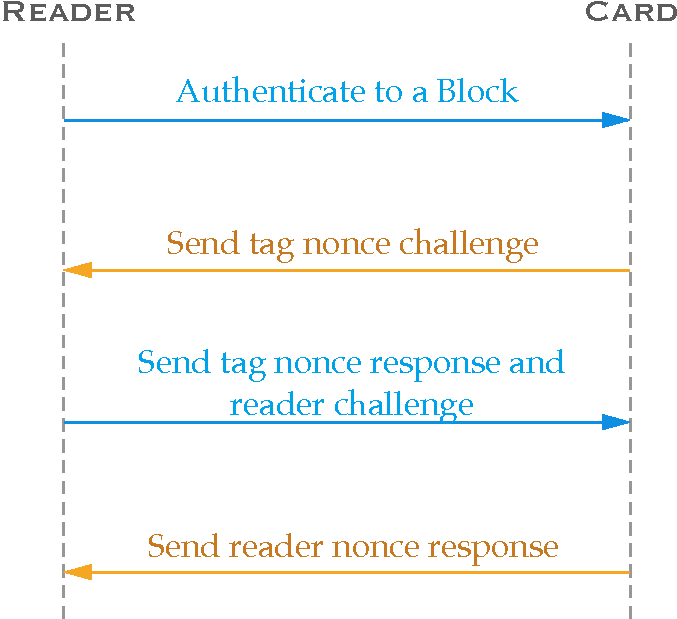
\includegraphics[width=0.4\textwidth]{three_pass_auth.pdf}
    \caption{Three Pass Authentication Handshake}\label{fig:three_pass_auth}
  \end{figure}


  The card/tag nonce is generated using a hardware pseudorandom number generator. The PRNG consists of a 32-bit linear feedback shift register (LFSR). On each clock cycle the leftmost bit is discarded and a new bit shifted in by XORing bits $16$, $18$, $19$ and $21$ as shown in Figure~\ref{fig:prng}.

  \begin{figure}[h]
    \centering
    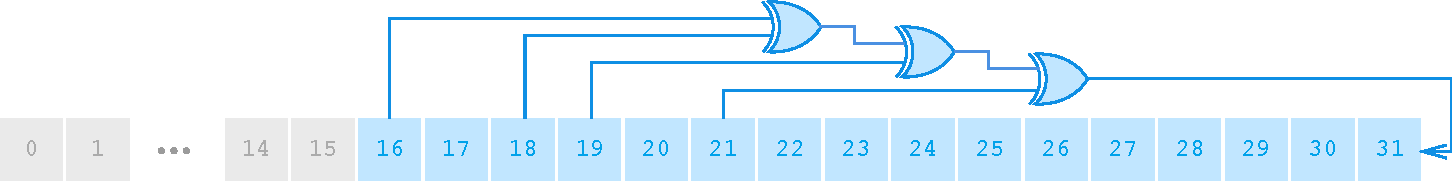
\includegraphics[width=0.9\textwidth]{prng.pdf}
    \caption{Pseudo Random Number Generator Schematic}\label{fig:prng}
  \end{figure}

  The LFSR is \SI{32}{bits} long and thus produces 32-bit nonces. However, as can be seen in Figure~\ref{fig:prng}, the feedback function only uses the 16 rightmost bits, restricting the entropy of the generated numbers to \SI{16}{bits}. Instead of being able to produce $2^{32}-1$ ($4,294,967,295$) different random numbers the PRNG can only produce $2^{16}-1$ ($65,535$).

  The \mifare{} Classic chip is powered by the electromagnetic field of the reader. The chip loses power when it is removed from the reader or if the field is turned off. When the chip loses power, the PRNG resets to a known state. An attacker can therefore accurately predict the ``random'' nonce values by resetting the card and then waiting a fixed number of clock cycles before requesting the nonce.

  \subsection{Parity Bits Leak Information}

  The ISO/IEC 14443-A standard requires that every byte of data transmitted be followed by a parity bit for transmission error detection. The parity bit specifies whether there is an even or odd number of ``1'' bits in the byte and thus allows detection of single bit transmission errors.

  The standard is agnostic about the data being transmitted and makes no specific provision for authentication or encryption. To introduce encryption in a way that is compliant with the standard, the parity bits should be added after the transmission data is encrypted. The \mifare{} Classic not only adds the parity bits prior to encryption but also encrypts them with the same bit of the keystream as is used for the next bit of the plaintext as shown in Figure~\ref{fig:keystream_reuse}. In general, this reduces the entropy of every byte transmitted by one bit as it leaks whether the first bit in a byte is the same as the parity bit of the previous byte.

  \begin{figure}[h]
    \centering
    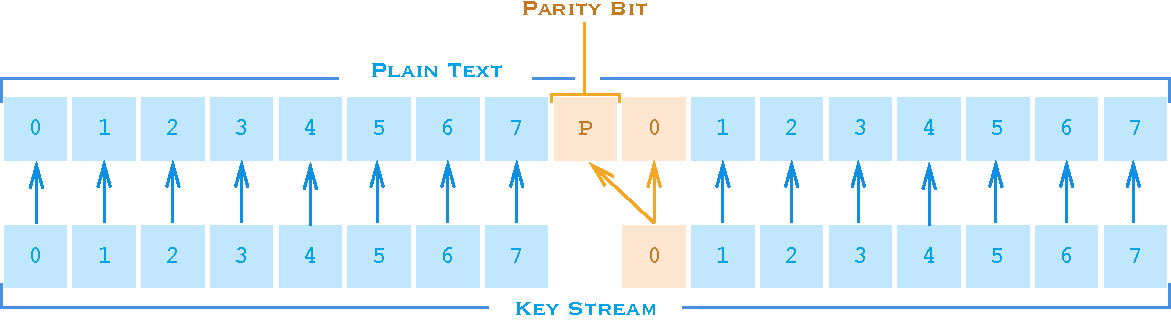
\includegraphics[width=0.9\textwidth]{keystream_reuse.pdf}
    \caption{Key Stream Bit Reuse on Parity Bits}\label{fig:keystream_reuse}
  \end{figure}

  During the authentication handshake shown in Figure~\vref{fig:three_pass_auth}, when the reader responds to the card nonce, the card verifies the parity bits before checking whether the response is valid. If the parity bits are incorrect, the card ceases communication. If all eight parity bits are correct, the card responds with a 4-bit error code. There are 8 parity bits and a randomly chosen parity bit has a $50\%$ chance of being correct. Therefore when choosing a response randomly, all 8 parity bits are correct with probability 1 in 256. The error code is encrypted despite the authentication failing, thus allowing the recovery of four bits of the keystream by XORing the received encrypted error with the known plaintext value.

  \subsection{LFSR Can Be Rolled Back}
  Communication between the card and the reader is encrypted with the proprietary encryption algorithm \crypto{}. A successful authentication handshake initialises the 48-bit \crypto{} linear feedback shift register (LFSR) in both the card and the reader. Note that this is a different LFSR than the one in the PRNG.\@

  \crypto{} is a stream cipher; at each clock cycle a keystream bit is generated from the LFSR using the filter function as shown in Figure~\vref{fig:lfsr}. The filter function is constructed using 3 smaller filter functions ($f_a$, $f_b$, $f_c$), each of which returns either a $1$ or a $0$ depending on the values of its inputs.

  Every clock cycle the LFSR shifts a bit to the left, discarding the leftmost bit and inserting a new bit from the feedback function by XORing several bits together as shown. The keystream bit is XORed with the next plaintext bit before transmission. Upon receipt of an encrypted transmission, the reader XORs each bit of the ciphertext with successive bits of the keystream to recover the plaintext.

  \begin{figure}[h]
    \centering
    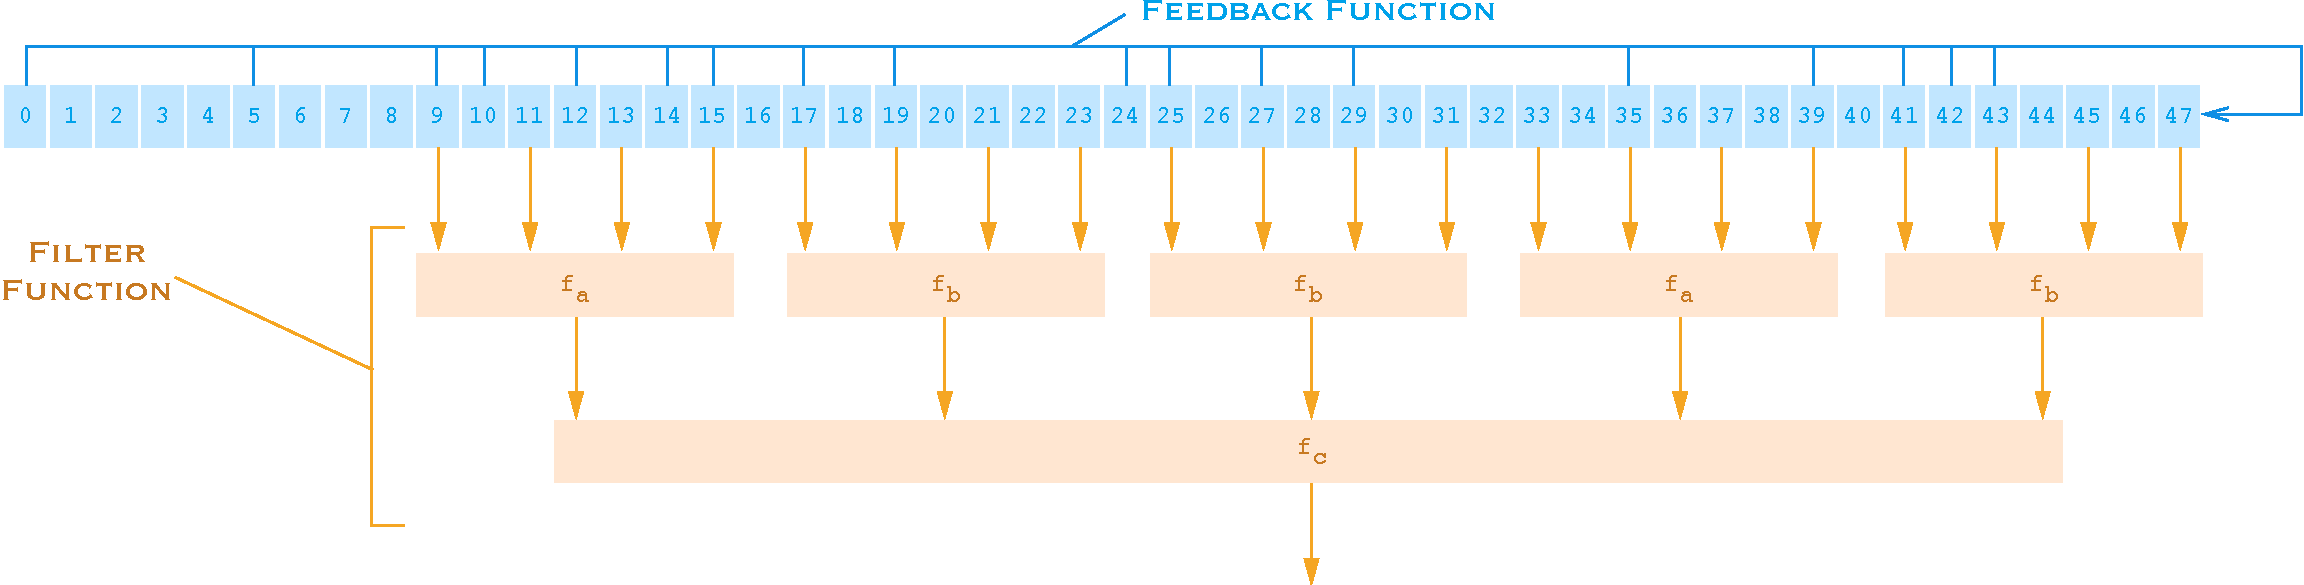
\includegraphics[width=\textwidth]{lfsr.pdf}
    \caption{\crypto{} LFSR Construction}\label{fig:lfsr}
  \end{figure}

  If the LFSR state is known then it can be rolled back, recovering both its initial state and all keystream bits. To roll back the LFSR state by one clock cycle, each bit is shifted one to the right. The value of the new bit (position $0$) can be determined by using the bit that we shifted out of position $47$. This bit was produced by XORing 18 bits together, 17 of which we know and the 18th is the new bit.

  \subsection{LFSR State can be Recovered}\label{sec:lfsr_state_recovery}
  As can be seen from Figure~\vref{fig:lfsr}, all the 20 input bits to the filter function are odd bits from the LFSR.\@ This allows an attacker that has recovered part of the keystream to invert the filter function and recover the LFSR state by doing the following:

  \begin{enumerate}
    \item Consider the first bit of the recovered keystream $ks_0$ and the LFSR bits that input into the filter function (bits $9$, $11$, \ldots, $47$). Compute all possible filter inputs that produce $ks_0$. The structure of the filter function guarantees that there will be exactly $2^{19}$ such possibilities.

    \item For each of the possibilities:
      \begin{enumerate}
        \item Shift the LFSR 2 bits to the left and consider the keystream bit 2 positions after the previous one. In other words, we iterate over either the even or odd keystream bits.

        The filter function still has 19 of the previous 20 bits as inputs and a new bit from the feedback function.

        \item The new bit could be either a $1$ or a $0$, check if each of these possibilities result in the correct keystream bit when put through the filter function.
          \begin{itemize}
            \item If neither result in the correct keystream bit, then this sequence of LFSR bits has been eliminated, so we remove it.

            \item If one results in the correct keystream bit, then this sequence of LFSR bits is extended with this new bit value.

            \item If both result in the correct keystream bit, then we duplicate the sequence and extend one sequence with a $0$ and one with a $1$.
          \end{itemize}
        \item We repeat this until we have run out of keystream bits. We now have a list of sequences of alternate LFSR bits, each of which produces the alternate bits of the keystream.
      \end{enumerate}

    \item Having recovered the LFSR sequences corresponding to the even bits of the keystream we now repeat this, starting with $ks_1$ to recover the sequences for the odd bits of the keystream.

    \item Combining the odd and even sequences provides candidate sequences for the entire LFSR state. To do this, the bits of the sequences are checked to see if they satisfy invariants that should hold due to the construction of the feedback function.
  \end{enumerate}

  The number of candidate states returned varies depending on how many keystream bits were used. When 32 bits are used, on average $2^{16}$ candidate states are returned. When 64 bits are used only one state is returned.


  \section{Attack}
  The weaknesses outlined in the previous section can be exploited via a range of attacks. This section describes one of the most effective attacks. The attack only requires access to a card and doesn't need specialist equipment.


  \subsection{Secret Key Recovery from Nested Authentication}

  When a reader with an existing authenticated session wants to re-authenticate to use a different secret key the protocol differs slightly and the three pass handshake shown in Figure~\vref{fig:three_pass_auth} is encrypted. Therefore, if we are able to predict the plaintext (tag nonce) it is possible to recover \SI{64}{bits} of keystream by XORing the plaintext with the ciphertext.

  The first sector on \mifare{} cards is readable with a default key and thus it is always possible to obtain an authenticated session with which to mount this attack.

  Due to the PRNG weakness, the nonces have at most 16 bits of entropy. The parity weakness further reduces this to just 6 bits and thus just 64 candidate nonces. Enumerating each possibility is feasible but in practice we can do better, as even the timing information from off-the-shelf readers is sufficient to determine roughly what state the PRNG is in and thus which of the 64 candidate nonces was most likely used.

  As described in Section~\vref{sec:lfsr_state_recovery}, the keystream bits can then be used to derive the LFSR state, which can be rolled back to its initial state, recovering the secret key.

  \subsection{Brute-Force Key Search}

  Prior to the reverse engineering of \crypto{} a brute-force attack had to be performed against the card directly. This required trying all possible 48-bit keys against the \mifare{} Classic card. The \mifare{} Classic specification~\cite{semiconductors2002mifare} states that the communication required to try a key should take a minimum of \SI{5}{ms}, it would therefore take in excess of \SI{40000}{years} to perform an exhaustive search on the entire keyspace.

  Now that the encryption algorithm has been reverse engineered, offline brute-force attempts can be carried out against captured communication with a card. The time required in an offline brute-force is inversely proportional to the cost. In 2009 a \$10,000 computer could crack DES (a much slower and more gate hungry algorithm) in a week~\cite{kumar2006breaking}. A 48-bit key is therefore insufficient to provide robust security with the computing resources available today, even with a better cipher.


  \section{Attack Countermeasures}

  In this section I explore various countermeasures to the above attacks, explaining both how they work and how they mitigate the risk of attack.

  \subsection{Digital Signature Protection}
  The security of the \mifare{} Classic card is compromised so severely that any data stored on the card no longer has data integrity or confidentiality. If the data corresponds to a balance then the weaknesses allow an attacker to commit fraud. Within the context of \UoC{}, an attacker could change the student identifier or CRSID to gain unauthorised access to buildings.

  Digital signatures provide cryptographic assurance of the integrity of the data, irrespective of the security of the card itself. Data signed with a robust digital signature algorithm cannot be created or modified without access to the signing key, as doing so would lead to an invalid signature.

  \subsubsection{Protection Against Cloning}
  Digital signatures do not provide any inherent protection against cloning. The presence of a valid signature provides nonrepudiation --- strong cryptographic assurance that the data was created by the signer. However, an adversary with read access can copy both the data and the signature to clone the card.

  \mifare{} Classic cards have a read only unique identifier (UID) that is set during manufacture. By also signing the UID an attacker won't be able to clone the data onto another \mifare{} Classic Card as the signature will be invalid.

  An attacker can bypass this, however, if they are able to set the UID.\@ Specialist hardware like the Proxmark 3 can emulate a \mifare{} Classic card with an arbitrary UID.\@

  \subsubsection{Requirements}
  The primary purpose of this dissertation is to explore countermeasures that organisations with existing \mifare{} Classic deployments can implement until they are able to migrate to a more secure card. Given this, it is desirable that any Digital Signature proposal meets the following criteria.

  \begin{itemize}
    \item \bold{Backwards Compatible} \\
      In the unlikely event that is was feasible to update all readers and cards in one go then the organisation could migrate to a more secure card instantly.

      In the more realistic scenario where readers and cards will be updated to incorporate digital signatures gradually, it is vital that the scheme is backwards compatible. Readers that have not been updated should not be affected and should continue to operate (without enhanced security).

    \item \bold{Agnostic of Card Structure} \\
      Different organisations structure the data on their cards in different ways. Even a single organisation may not have a structure that is consistent across all cards. The digital signature implementation should be flexible enough to work with all typical deployments rather than being specific to any one card layout.

    \item \bold{Allow Key Updates} \\
      Whilst every effort should be made to prevent the private keys from being leaked, it would be foolish to not plan for this eventuality. Following a breach the private keys should be changed, and the system should be able to deal with this in a way that minimises disruption.

    \item \bold{Support Multiple Signatures} \\
      A single card may contain data from different sub-organisations, each of which may want to add a signature. For example, within \UoC{}, central university may wish to sign some data such as the student ID and expiry date. This should not preclude colleges from signing their own data independently.
  \end{itemize}


  \subsection{Key Diversification}

  Without key diversification, every card within a deployment has the same set of secret keys. Should an attacker be able to extract the secret keys from one card they will be able to use them to access any other card within the deployment. With key diversification, the secret keys for a particular card are cryptographically derived from a master key using the unique ID of the card.

  With key diversification an attacker is forced to extract the secret keys from any card they wish to clone. Instead of requiring a few seconds of communication with the target card the attacker may require several minutes to extract all 80 keys of a 4K card. It would be harder for an attacker to sustain this prolonged access covertly.


  \subsection{Interaction Counter}

  Key diversification makes it more challenging but not impossible for an attacker to dump the data from a card. Digital signature protection makes it harder for an attacker to use dumped data to create a clone as the UID of the card is signed. Neither of these, however, make it impossible. It is thus desirable to be able to detect the presence of cloned cards.

  By using an interaction counter it is possible to detect the use of some cloned cards. The counter consists of an integer and occupies one 16-byte block. When the card is placed on a reader, the counter is incremented. Networked readers report the current value to a central system. The central system checks that any counter value reported is more than the previously highest reported value for that card. When a card is cloned, if either the original or the clone is used, the counter in each gets out of sync and thus when the other card is used the counter value will be less than the previously reported value, indicating that the card is cloned.

  Whilst this method won't detect all cloned cards, the possibility of detection would act as a deterrent.

  \subsubsection{Limitations}

  This does not protect against the situation where the owner of the cloned card is complicit in its cloning. If this is the case then the counters can be kept in sync.

  When a reader detects the presence of a clone it doesn't know whether the current card is the clone or the cloned card. It may be undesirable therefore to reject access.

  Only networked readers can report cloned cards, however non-networked ones can still increment the counter, allowing detection by subsequent access to an online reader.

  \subsection{Emulated Card Detection}
  With the proposed digital signature protection, an attacker not only has to clone the contents of the card but also the UID.\@ The UID in \mifare{} Classic cards cannot be changed. An attacker therefore has to either obtain a knock-off card that allows changing the UID or emulate the card using a device such as the Proxmark 3.

  Recall that \mifare{} Classic cards have a hardware based random number generator (PRNG) used to generated nonces. Also recall that the PRNG is flawed as the feedback function only takes input from the rightmost 16 bits as shown in Figure~\vref{fig:prng2} resulting in the generated 32-bit numbers having at most \SI{16}{bits} of entropy.

  \begin{figure}[h]
    \centering
    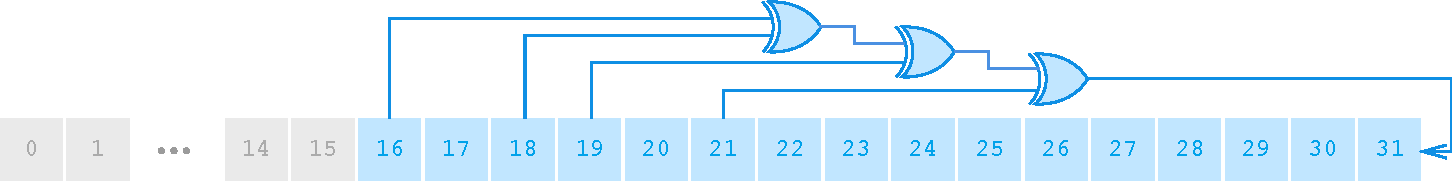
\includegraphics[width=0.9\textwidth]{prng.pdf}
    \caption{Pseudo Random Number Generator Schematic}\label{fig:prng2}
  \end{figure}

  Most emulators do not implement a firmware/software version of the \mifare{} Classic's PRNG and instead use their own source of random nonces. The random nonces generated by the PRNG are used in the initial authentication handshake between the card and the reader as shown in Figure~\vref{fig:three_pass_auth}.

  Since the hardware PRNG can only generate $2^{16}-1$ (\SI{65535}{}) different nonces it is easy to check whether a given nonce could have been generated by the PRNG.\@ This allows the reader to accurately identify emulated cards that don't use the same PRNG.\@ The reader can then reject access and flag for review.

  \subsubsection{Limitations}

  Assuming the nonces generated by the emulated card are uniformly picked at random from all $2^{32}-1$ possibilities, there is a one in \SI{65535}{} chance that it will be in the PRNG range and thus be indistinguishable, using this method, from a genuine \mifare{} Classic Card.

  Given the weakness in the PRNG is a hardware implementation flaw rather than a weakness in the authentication protocol it is possible that NXP could fix the flaw in the PRNG in future cards in a backwards compatible way. If the readers were programmed to reject these cards then this would cause disruption.

  I am of the opinion that it is unlikely that NXP will alter the implementation. The cards have been produced for eight years since the weaknesses were published and NXP have yet to make a change. The \mifare{} Classic protocol is fundamentally broken and whilst fixing the PRNG would mitigate some of the attacks, it would not prevent all of them.

  \section{Card Revocation}
  Cards are often issued with an expiry date after which they can no longer be used. Without digital signature protection, an adversary can use the attacks previously described to change this expiry date, potentially allowing them to gain unauthorised access. By including the expiry date in the data to be signed, an attacker cannot use an expired card simply by changing the expiry date.

  There are a variety of circumstances under which it is necessary (or at least highly desirable) to revoke a card before its originally planned expiry date. Within the context of \UoC{}, reasons for revoking a card early include:

  \begin{itemize}
    \item The card is lost, stolen or broken
    \item A student or member of staff leaves early
  \end{itemize}

  In this section I outline some existing solutions, explain their shortcomings when applied to \mifare{} Classic deployments and propose a card revocation system that uses the cards to distribute a list of revoked cards from online (networked) readers to offline (non-networked) readers.

  \subsection{Existing Solutions}
  \subsubsection{Revoke Card in Central Database}

  Networked or ``online'' card readers query a central database each time a card is presented. Revoking access via these readers is thus simply a case of updating this central database to either remove the card or mark it as revoked.

  There are a variety of factors that may make the installation of a networked reader impractical. Within \UoC{}, offline door-access readers (those without a network connection) are common. Currently, to revoke access to these readers, they have to be manually updated. The resources required to update each offline reader when a card is lost are sufficiently high that it is seldom done, resulting in lost or stolen cards remaining active.

  \subsubsection{Hotel Key-Card Solution}
  Some hotels issue key-cards to access rooms. The door to the room has an integrated, unnetworked reader. The hotel solution relies on each card only having access to a single reader and cannot easily be extended to an arbitrary network of readers and cards.

  If a guest checks out or loses their room key then the hotel issues a new key and revokes the old one. This usually works by incrementing a per-room counter stored on the card each time a new one is issued. The reader maintains its own counter that it updates whenever a card with a higher counter is used. The reader reject cards with a counter lower than their internal one. Therefore the act of using a new card automatically revokes previously issued ones.

  Within the context of a hotel this scheme has several benefits:
  \begin{itemize}
    \item \bold{No network or power required} \\
      It would be expensive to run a network connection to each door in the hotel so there are significant cost savings by removing the need for one. The readers only require a very small amount of power and can usually run for years from a small integrated battery.

    \item \bold{Guests can extend their stay} \\
      If a guest extends their stay their card will continue to work.

    \item \bold{Multiple cards can be issued} \\
      Multiple cards can be issued to guests by issuing cards with the same counter value. If a second guest staying in the room arrives later then a second card can be issued with the same counter value without reissuing the previous cards.

  \end{itemize}

  \section{Card Revocation Gossip Protocol}
  Whilst offline readers aren't networked in a traditional sense, they are part of a network of readers through which cards travel. Cards can be used as a medium to transfer data between readers and thus can be used to distribute a list of revoked cards from online readers to offline ones.

  \subsection{Requirements}
  The card revocation protocol is for use in deployments with a mixture of networked and non-networked readers, such as \UoC{}. The protocol distributes the revocation list to offline readers, using the cards as a medium for communication. The network is unreliable and unpredictable and the protocol should be tolerant of this, making specific provisions for:

  \begin{itemize}
    \item varying numbers of online and offline readers
    \item different network topologies
    \item varying numbers of cards
    \item varying numbers of revoked cards
  \end{itemize}

  \subsection{Development Model}
  Given the importance of the protocol performance, and the unpredictable nature of large scale simulations, an iterative approach to development is appropriate. This allows changes to the protocol that are motivated by particular areas of poor performance.

  \subsection{Simulation Suite}
  A suite that simulates a network of readers and cards in varying configurations is necessary to assess the performance of each implementation. It is of significant benefit to use the simulation suite during development to highlight particular situations under which the implementation performs poorly and inform changes.

  \section{\mifare{} Libraries}
  In order to implement the digital signatures and card revocation gossip protocol it is necessary to be able to communicate with a \mifare{} Classic card. After investigating the viability of using an existing \mifare{} library I decided that writing my own would be preferable for reasons outlined below.

  Both Windows and OS\,X have built in ``smart-card'' APIs for interacting with both contactless and contact smart-cards. Using either of these APIs would make my implementation platform-dependent, something I wanted to avoid. Both APIs are also reasonably high-level and don't expose sufficient   low-level functionality to implement all of my proposed countermeasures.

  Libnfc is an open source C library with support for a variety of NFC cards and readers. Libnfc is cross-platform and exposes enough of the low-level functionality of the cards to implement all of my proposed protections. It would have been possible to implement my project entirely in C using libnfc. The decision to write my own library in the Go programming language has several benefits and was motivated by a variety of factors:

  \begin{itemize}
    \item \bold{Go is a high level language} \\
      Go is an object orientated, garbage collected, high-level language, which makes writing and maintaining certain aspects of the implementation easier.

    \item \bold{Ability to write unit tests} \\
      It is a well established software-engineering practice to write unit tests for code. Had I written the software directly on top of libnfc, it would have been prohibitively difficult to write tests that didn't depend on a physical card. By writing my own library I'm able to provide sufficient abstraction to allow mock versions of hardware readers and cards for tests.

    \item \bold{Ability to write simulations to benchmark} \\
      It would be impossible to write the simulation suite on top of libnfc. By writing my own library I can write code that works with both simulated readers and cards as well as physical ones.

    \item \bold{Suitability of Go} \\
      Go was chosen as the language to implement the core library in for a variety of reasons including:
      \begin{itemize}
        \item The project makes extensive use of cryptographic operations and Go has excellent support for these in its standard library
        \item The asynchronous nature of NFC communication is a natural fit for Go's concurrency primitives such as goroutines and channels.
        \item Go can be cross compiled to produce statically linked binaries for all major platforms.
      \end{itemize}

    \item \bold{Would provide a significant contribution to the community} \\
      Many of the potential problems I faced with using libnfc directly also affect others developing software for \mifare{} Classic cards. By releasing an open source library I will have made a substantial contribution to the community.
  \end{itemize}


\end{document}
